\begin{figure*}[t]
  \centering
  \begin{subfigure}[t]{0.18\textwidth}
    \centering
    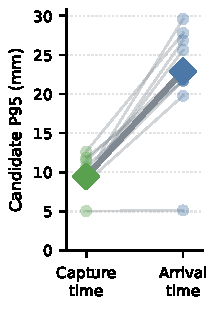
\includegraphics[width=\linewidth]{figures/panels/figure3a_capture_alignment.pdf}
    \caption{采集时刻对齐}
    \label{fig:exp2-alignment}
  \end{subfigure}\hfill
  \begin{subfigure}[t]{0.18\textwidth}
    \centering
    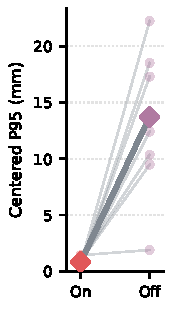
\includegraphics[width=\linewidth]{figures/panels/figure3b_static_lock.pdf}
    \caption{StaticLock}
    \label{fig:exp2-static-lock}
  \end{subfigure}\hfill
  \begin{subfigure}[t]{0.18\textwidth}
    \centering
    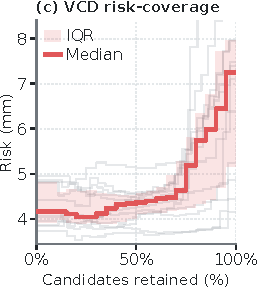
\includegraphics[width=\linewidth]{figures/panels/figure3c_vcd_risk_coverage.pdf}
    \caption{VCD score 风险--覆盖率}
    \label{fig:exp2-vcd}
  \end{subfigure}\hfill
  \begin{subfigure}[t]{0.40\textwidth}
    \centering
    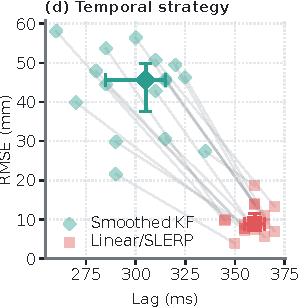
\includegraphics[width=\linewidth]{figures/panels/figure3d_temporal_strategies.pdf}
    \caption{时序策略}
    \label{fig:exp2-temporal}
  \end{subfigure}
  \caption{实验二的组件归因与逐帧输出策略比较。图~(a)、(b) 分别比较采集时刻复合和 StaticLock；图~(c) 展示 VCD 分数诱导的 event 级风险--覆盖率：从高 VCD 候选逐步加入低 VCD 候选，横轴表示保留候选比例。图~(d) 的主体是 Smoothed KF Extrapolation 与 Linear/SLERP，Hermite 为补充条件。三路均关闭 StaticLock，并共享模型、接纳、生命周期、候选序列和渲染时间线。为比较可读性，图~(d) 不显示超过 32~mm 的异常片段，完整数值保留在绘图审计表中。}
  \label{fig:exp2-final}
\end{figure*}
